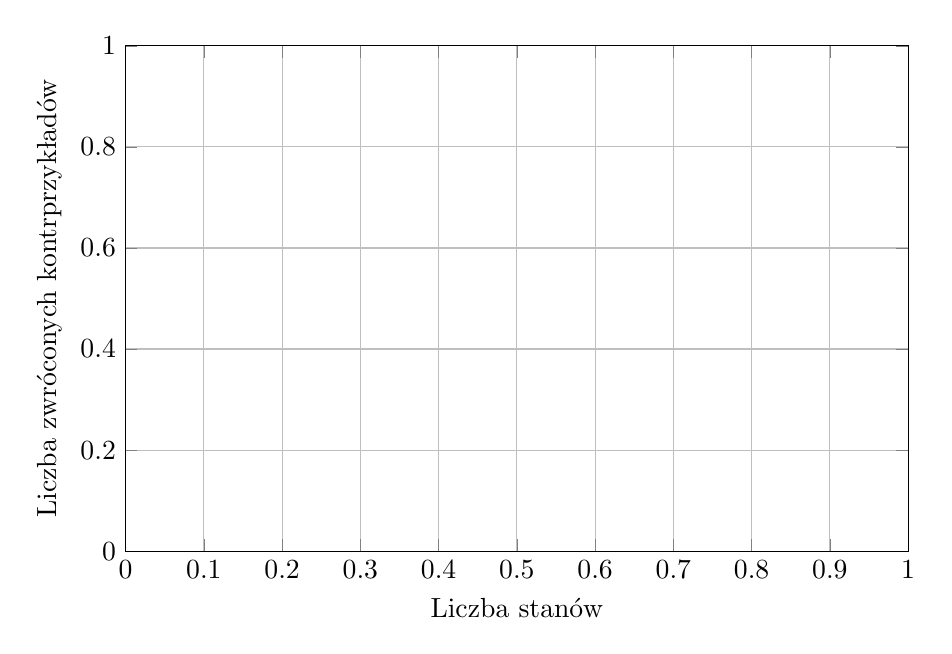
\begin{tikzpicture}
\begin{axis}[
    width=0.95\linewidth,
    height=8cm,
    xlabel={Liczba stanów},
    ylabel={Liczba zwróconych kontrprzykładów},
    grid=major,
    legend style={at={(0.02,0.98)}, anchor=north west, font=\small},
    legend cell align=left,
    xmin=2, xmax=32,
    enlargelimits=false
]
    \addplot[mark=*] coordinates { \DataCexSrs };
    \addlegendentry{Kontrprzykłady znalezione przez SRS}

    \addplot[mark=square*] coordinates { \DataEqNoSrs };
    \addlegendentry{Liczba zapytań $EQ$ bez SRS}

    \addplot[mark=triangle*] coordinates { \DataEqSrs };
    \addlegendentry{Liczba zapytań $EQ$ z SRS}
\end{axis}
\end{tikzpicture}